\section{Tree-Based Agentic Reasoning}
\label{sec:tree_based_agentic_reasoning}

% %!TEX root = ../../main.tex

\begin{figure}[!t]
    \centering 
    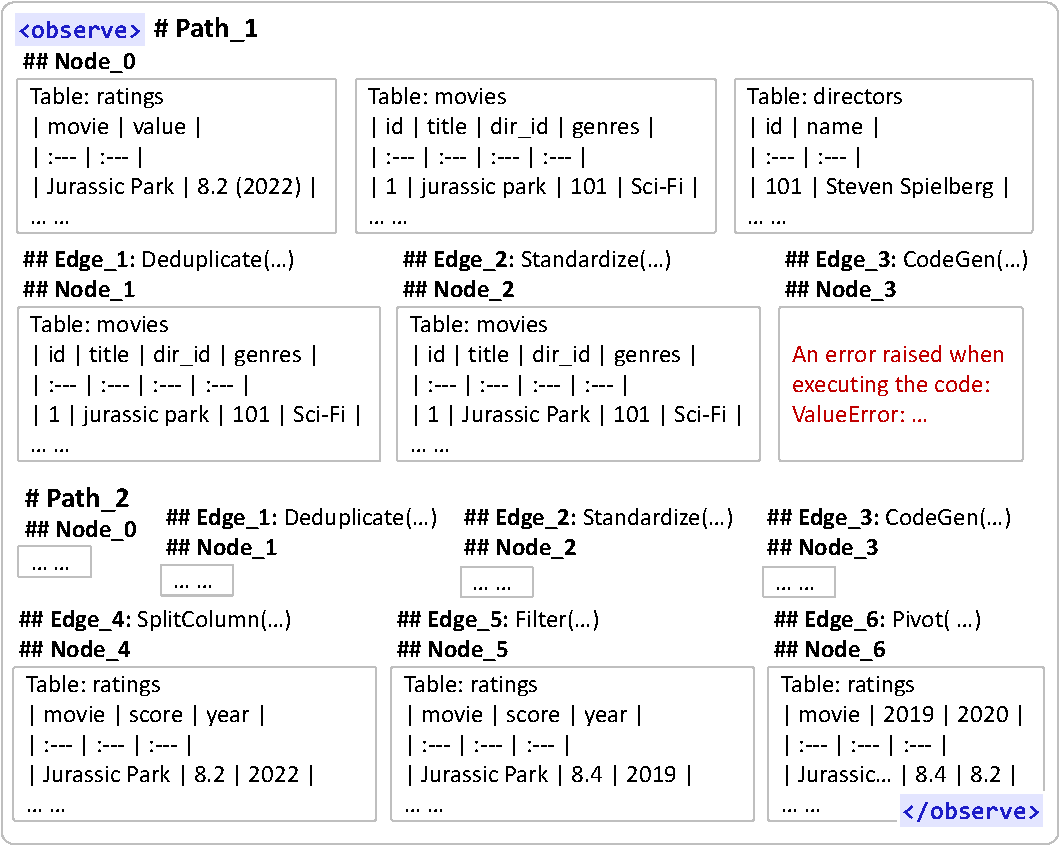
\includegraphics[width=1.01\columnwidth]{figures/fig/agentic_reasoning_observe.pdf}
    \vspace{-1em}
    \caption{An example of observe tag.
    }
    \label{fig:agentic_reasoning_observe}
    \vspace{-1em}
\end{figure}
%!TEX root = ../../main.tex

\begin{figure}[!t]
    \centering 
    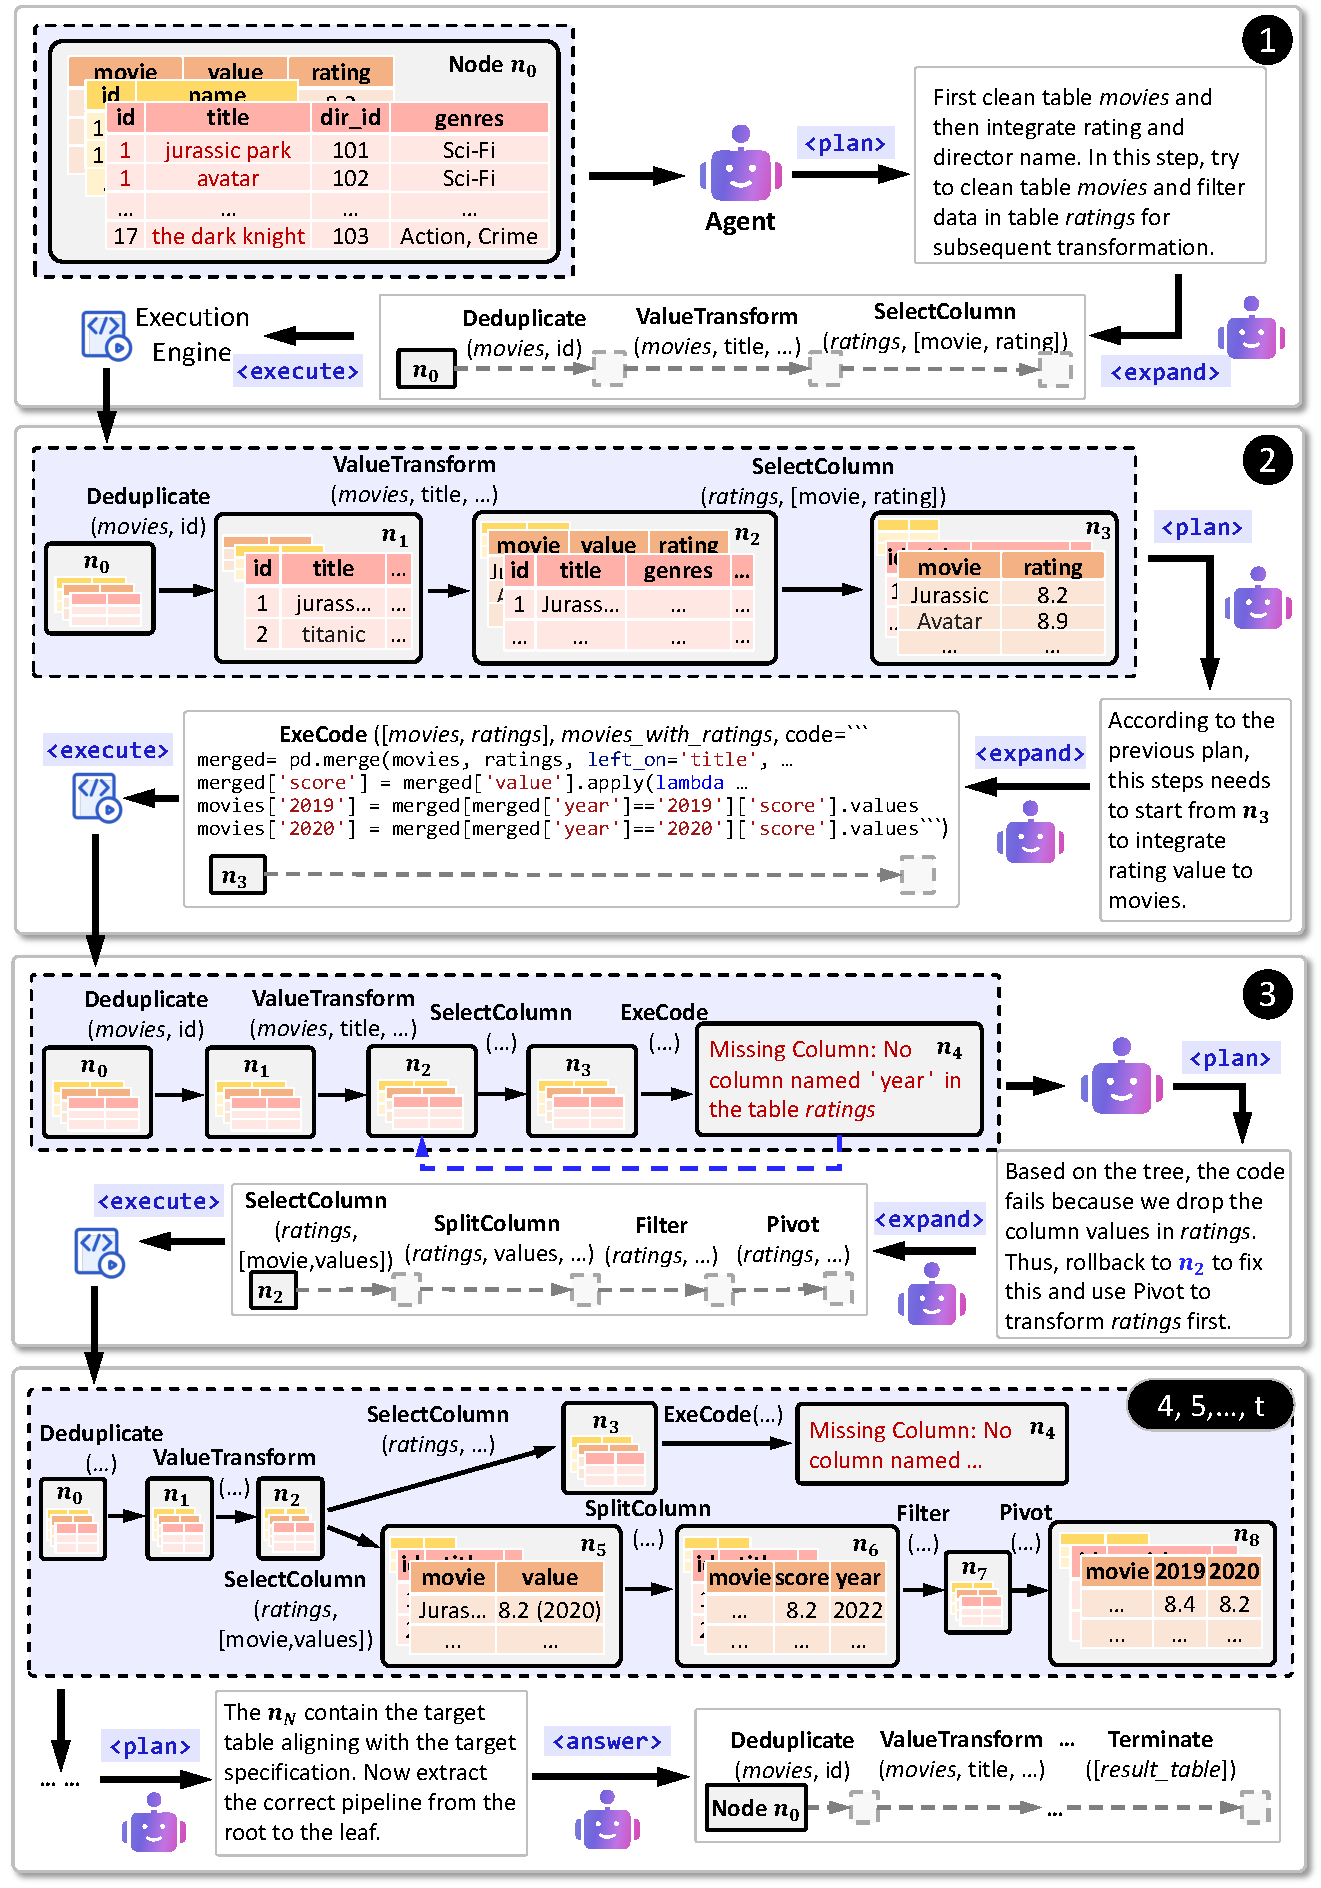
\includegraphics[width=0.99\columnwidth]{figures/fig/agentic_reasoning_example.pdf}
    \vspace{-1em}
    \caption{An example of tree-based agentic reasoning.
    }
    \label{fig:agentic_reasoning_example}
     \vspace{-1.5em}
\end{figure}

% As discussed in Section~\ref{sec:overview}, the sequential nature of ADP is inherently prone to \emph{irreversibility} (Challenge C1).
% Standard agentic frameworks, such as linear ReAct-style reasoning~\cite{yao2023react}, typically model the process as a linear chain where the environment state at step $t+1$ is derived solely from step $t$, \ie $\mathcal{T}_{t+1} = \text{Exec}(\mathcal{T}_t, o_t)$.
% This linear topology is insufficient for data preparation because many operators (\eg filtering, projection, and aggregation) cause permanent information loss.
% Once a destructive operator is executed, the previous state of the environment is overwritten. If the decision was suboptimal, the agent cannot recover the lost information to correct its course, leading to error propagation.

% \begin{example}
% Consider the task in Figure~\ref{fig:introduction_example}, where the goal is to report average ratings by genre.
% A crucial step is to apply \texttt{Explode} on the \texttt{genres} column (\eg splitting ``\{Sci-Fi, Action\}'' into distinct rows).
% If the agent overlooks \texttt{Explode} and directly orchestrates an aggregation (\eg \texttt{GroupBy} on \texttt{director} and \texttt{genres}), the multi-genre cell is treated as an atomic string.
% This results in an incorrect table where ratings for ``Sci-Fi'' and ``Action'' are merged into a non-existent category.
% In a linear rollout, this error is fatal: the agent only possesses the aggregated table, which lacks the granularity required to recover the individual genre associations.
% \end{example}

% To address this, we formalize the data preparation process as a search over a \textbf{Physical Execution Tree}.
% This structure decouples exploration from commitment, allowing the agent to branch out from any valid data environment, backtrack from errors, and systematically converge to the target schema.

% 冒段要解释我们提出了两个机制，一个是树，一个是reasoning，怎么解决了LLM在树上推理
% 树的定义篇幅少一些
% 机制怎么formal一些，***
%   - 参考（Graph），在tag前插入一个总体的机制公式（三小节，树，reasoning，example）
%   - 

To construct data preparation pipelines under complex dependencies and execution feedback, \sys employs a \emph{tree-based agentic reasoning} mechanism that supports structured exploration and non-local backtracking.
Specifically, we introduce an \emph{agentic reasoning tree} (Section~\ref{subsec:global_reasoning_tree}) that explicitly preserves historical states and alternative data preparation pipelines.
%allowing the agent to revise earlier decisions in response to execution failures or preparation mismatches rather than continuing from unpromising states.
Building on this tree structure, we define a tree-based agentic inference procedure (Section~\ref{subsec:agentic_tree_based_definition}) through a set of explicit agentic interaction actions. These actions specify how the LLM observes the current tree state, proposes data preparation plans, and generates promising pipelines.

%To address the limitations of linear reasoning in complex data preparation tasks, we propose a \emph{Tree-Based Agentic Reasoning} framework. This framework relies on two synergistic mechanisms to enable structured exploration and backtracking:
%(1) A \emph{Global Reasoning Tree}, which explicitly maintains the history of environment states (intermediate tables), allowing the system to preserve valid partial solutions and recover from failures.
%(2) A \emph{Structured Interaction Protocol}, which formalizes the reasoning process. This protocol guides the LLM to traverse the tree by strictly defining how to observe the current state, synthesize plans, and orchestrate operators within a unified generative process.
    
\subsection{Agentic Reasoning Tree}
\label{subsec:global_reasoning_tree}

We define the \emph{agentic reasoning tree} as a directed tree $G=(N,E)$, which represents the structured search space of pipeline construction starting from the initial source tables $\mathcal{S}$.
%
\begin{itemize}[leftmargin=1em]
    \item \textbf{Node ($N$).}
    Each node $n \in N$ corresponds to an \emph{environment state}, represented by the current set of intermediate tables maintained by the environment. In particular, the root node $n_0$ represents the initial state initialized with the source tables $\mathcal{S}$.
%
    \item \textbf{Edge ($E$).}  
    A directed edge $e=(n_i \xrightarrow{o} n_j) \in E$ represents a state transition induced by executing an \emph{operator instance} $o$ (\ie an operator type with specific parameters) orchestrated by the agent at state $n_i$. Specifically, executing $o$ updates the environment state from $n_i$ to $n_j$, yielding updated intermediate tables. 
\end{itemize}
%
In the agentic reasoning tree, each edge corresponds to a single operator instance, while a path from a node to another node represents an operator sequence, \ie a data preparation pipeline. 
%Take the agentic reasoning tree in Figure~\ref{fig:agentic_reasoning_example} as an example. In step 4, the tree comprises seven nodes and six edges, featuring two distinct branches diverging from node $n_2$.

% \fanj{give a brief example.}

%We define the \emph{Agentic Reasoning Tree} as $\mathcal{G}=(\mathcal{N}, \mathcal{E})$, which encapsulates the agent's exploration trajectory starting from the initial source tables.
%
%\begin{itemize}[leftmargin=1em]
%    \item \textbf{Node ($\mathcal{N}$).} Each node $n \in \mathcal{N}$ represents a distinct snapshot of the \emph{environment state}. This state primarily consists of the set of intermediate tables $\mathcal{T}$ currently maintained by the environment. The root node $n_0$ corresponds to the initial environment state containing the source tables $\mathcal{S}$.
%
%    \item \textbf{Edge ($\mathcal{E}$).} A directed edge $e=(n_i \xrightarrow{op} n_j) \in \mathcal{E}$ represents a state transition triggered by submitting an operator $op$ (orchestrated by the agent) to the environment at state $n_i$. The environment executes the operator and updates its internal state to $n_j$.
%\end{itemize}

%\subsection{Agentic Reasoning over Tree Structure}
\subsection{Tree-Based Agentic Inference}
\label{subsec:agentic_tree_based_definition}

The basic idea of our tree-based agentic inference is to develop an iterative decision-making process through a structured LLM interaction pattern.
Specifically, the LLM autonomously generates agentic \emph{interaction actions} to operate over a materialized agentic reasoning tree, incrementally expanding, revising, or backtracking tree branches based on execution feedback.
%This section presents the tree-based inference framework, defines the agentic actions, and describes the iterative inference procedure.

\stitle{Agentic Inference Framework.} 
Given source tables $\mathcal{S}$ and a target schema $\Sigma^\ast$, the framework produces a reasoning trajectory $R$ and finally generates an answer $A$ based on $R$.
More formally, we model this process by a probabilistic model $\Prob(\cdot)$ over the reasoning process and the answer generation conditioned on the inputs: 
\begin{equation}
\label{eq:overall_agentic_inference}
\Prob(A,R \mid S,\Sigma^*) = 
\underbrace{\prod_{t=1}^{T} \Prob(R_t \mid R_{<t}, S, \Sigma^\ast)}_{\text{Reasoning Process}} 
 \cdot 
\underbrace{\Prob(A \mid R, S, \Sigma^*) \vphantom{\prod_{t}^{T}}}_{\text{Answer Generation}}.
\end{equation}
where $T$ denotes the length of the reasoning process and $R_t$ represents the reasoning results of the agent at step $t$.

The reasoning process is implemented by adopting an LLM-based agent to search over the agentic reasoning tree $G$ in a generative way. Specifically, the process alternates in an iteration of \textit{plan}, \textit{expand} and \textit{execute} steps where it generates logical plans for the current step based on the observation of the current tree, expands new branches and execute expanded operators to update the current tree. Based on this idea, we break the step-wise reasoning process in Eq.~(\ref{eq:overall_agentic_inference}) down into the following formula.
\begin{equation}
% \nonumber
\label{eq:reasoning_process}
\begin{split}
&  \Prob(R_t | R_{<t}, S, \Sigma^\ast) =  \\
\underbrace{\Prob_{\text{LLM}}(\psi_t | \psi_{<t}, G_{t-1}, \Sigma^\ast)}_{\action{plan}} 
& \cdot
\underbrace{\Prob_{\text{LLM}}(\mathcal{P}_t | G_{t-1}, \psi_{t})}_{\action{expand}}
\cdot
\underbrace{\revise{\mathtt{Env}}(G_t | G_{t-1}, \mathcal{P}_t)}_{\action{execute}}.
\end{split}
\end{equation}
where $\Prob_{\text{LLM}}$ denotes the generative distribution induced by the LLM agent, $\psi_t$ and $\mathcal{P}_t$ denotes the logical plan and expanded operator pipeline generated by the agent in step $t$, and \revise{$\mathtt{Env}$} represents the environment transition distribution that materializes $\mathcal{P}_t$ to get an updated agentic reasoning tree $G_t$.

% After $T$ steps of reasoning process defined in Eq.~(\ref{eq:reasoning_process}), we generate a complete operator pipeline as the final answer $A$.

\stitle{Actions for Agentic Inference.} We regulate this interaction using control tags aligned with the components in Eq.~(\ref{eq:overall_agentic_inference}) and Eq.~(\ref{eq:reasoning_process}).

% \stitle{Agent Tags.}
% To regulate the interaction between the agent and the environment, we introduce a set of structured tags. These tags formalize the protocol for observation, planning, and orchestration.

\begin{itemize}[leftmargin=1em]
    % \item \action{observe}.
    % This tag encapsulates the system-generated observation.
    % We serialize the Global Reasoning Tree $\mathcal{G}$ into a textual prompt $p$, formatting table schemas and data samples in Markdown.
    % % \underline{Highlight:}
    % To mitigate the context window constraints of LLMs, we implement a differential strategy.
    % While the root node $n_0$ is fully serialized, for any subsequent node $n_i$ ($i>0$), we only serialize the tables within the environment that were modified by the incoming operator.
    % This preserves the semantic continuity of the transformation flow, allowing the agent to focus on incremental changes (\eg how a \texttt{Join} alters the schema) rather than redundant static data.

    \item \action{plan}.
    This action produces a high-level logical plan for the next reasoning step.
    Given the current agentic reasoning tree, the target schema $\Sigma^\ast$, and prior plans, the agent generates a plan $\psi$ that specifies the intended reasoning decision.
    The plan analyzes the current environment state to determine whether to continue expanding the tree or terminate the reasoning process. If further exploration is required, it identifies the parent node to extend and the candidate operations to apply. 
    % \revise{Notably, since the tree preserves failure states with their error traces, the plan can leverage this historical failure information to avoid repeating previously unsuccessful attempts.}
    %This tag delimits the agent's reasoning phase. 
    % At step $t$, the agent first observes the current agentic reasoning tree $G_{t-1}$ and refer to previous plan $\psi_{<t}$ to generate a logical plan $\psi_t$ to guide the next expanding actions.
    %Based on the observation of the current agentic reasoning tree, the target schema $\Sigma^\ast$, and previous plans, the agent generates a high-level logical plan $\psi$.
    %Specifically, the plan analyze the environment state to determine whether to expand new branch or terminates the reasoning process. If the tree requires further exploration, the plan will identify which node should be the father node and what operations should be expanded.
    % It contains not only the 
    % The planning is structured into two levels: First, it determines whether to \texttt{terminate} or \texttt{expand}; and (2) \emph{Tactical Execution}, identifying the parent node (environment state) and the intended logic for the next step.
    % \underline{Highlight:}
    % We retrieve the top-$k$ most relevant past logical plans from memory $M$ to prevent the agent from repeating previous mistakes and plan at a global perspective.
    % The planning is structured into two levels: (1) \emph{Strategic Decision}, determining whether to \texttt{terminate} or \texttt{expand}; and (2) \emph{Tactical Execution}, identifying the parent node (environment state) and the intended logic for the next step.
    % This hierarchical approach mitigates the ``lost-in-the-middle'' phenomenon common in long-horizon reasoning.

    \item \action{expand}.
    This action generates a candidate operator pipeline expanded from a selected parent node $n_{\texttt{parent}}$. Conditioned on the plan $\psi$, the agent produces an operator sequence $\mathcal{P}$ to extend node $n_{\texttt{parent}}$. To ensure consistent node selection, the parent node is specified using a prefix-matching constraint: the agent must reference the full operator sequence from the root to that node. This constraint avoids ambiguous or index-based node references and enforces alignment between the proposed expansion and the recorded transformation history.

    %Guided by plan $\psi$, the agent synthesizes a candidate operator pipeline $P$ expanded from $n_{\text{parent}}$.
    %To avoid hallucination in node selection, we enforce a {prefix-matching strategy}: the agent must reference the operator sequence from the root to uniquely identify $n_{\text{parent}}$.
    %This design mitigates risks of arbitrary numerical indexing (\eg predicting ``Node 5''). By regenerating the operator lineage, the agent must attend to the transformation history, providing a {verification step} that aligns its actions with the actual state of the chosen parent rather than a disconnected or hallucinated node ID.
    % Furthermore, we incorporate an {early-stop mechanism}: if any operator in $\Delta \Pi$ triggers an execution exception within the environment, the expansion halts immediately, and the node is tagged with the error trace to prune the invalid branch.
    

    \item \action{execute}. 
    This action applies the candidate operator pipeline through the environment and performs state transitions. Specifically, given a candidate pipeline $\mathcal{P}_t$, the environment executes its operators sequentially over the materialized tables at the selected parent node. After each operator is successfully applied, a new intermediate state node is created to store the resulting tables, and a directed edge is added from the previous state node to the new one. Repeating this process for all operators in $\mathcal{P}_t$ yields a chain of new nodes, which updates $G_{t-1}$ to $G_t$.
    % This action applies the candidate operator pipeline through the environment and performs state transition. Specificially, given a candidate pipeline $\mathcal{P}_t$, the environment executes its operators sequentially over the materialized tables at the selected parent node. If execution succeeds, a new child node $n_{\text{new}}$ is created with the resulting intermediate tables, and a directed edge is added to update the reasoning tree from $G_{t-1}$ to $G_t$. 
    If execution fails due to a runtime exception (\eg column mismatch or type error), no new state node is created; instead, the parent node is annotated with a failure state that records the error trace. 
    % \revise{These failure annotations are serialized into the prompt for subsequent reasoning steps, enabling the agent to recognize and avoid repeating the same errors when generating new branches.}
    
%    This tag represents the deterministic state transition triggered by the environment, corresponding to $P_{\text{Env}}$ in Eq.~(\ref{eq:reasoning_process}).
%    Upon receiving the candidate pipeline $P_t$, the environment executes the operators sequentially against the materialized tables at the parent node.
%    If execution succeeds, a new child node $n_{new}$ is instantiated containing the resulting intermediate tables, and a directed edge is added to $G_{t-1}$ to form $G_t$.
%    Conversely, if an operator triggers a runtime exception (\eg column name mismatch or type error), the execution halts immediately.
%    In this scenario, the environment does not create a valid state node but instead annotates the parent node with a \emph{failure edge} containing the error trace.
%    This immediate feedback mechanism acts as a pruning signal, preventing the agent from further exploring invalid branches.
    \item \action{answer}.
    This action terminates the reasoning process and returns the final pipeline.
    It is triggered when a leaf node state satisfies the target schema $\Sigma^\ast$.
    The root-to-leaf operator path associated with that node is extracted as the final pipeline $\mathcal{P}^\ast$.
    % and returned as the output.
%
%    This tag signals task completion.
%    It is triggered when the agent verifies that a leaf node's environment state satisfies the target schema $\Sigma^\ast$, extracting the path from the root to this leaf as the final pipeline $\Pi$. We output $\Pi$ as the answer.

    % \underline{Highlight:}
    % For complex tasks where the exploration budget is exhausted without a perfect match, this tag supports a ``last-mile'' capability. It allows the agent to output a pipeline $\Pi$ that extends the current best path with speculative, unverified operators, ensuring the system always returns a best-effort solution.
\end{itemize}

\stitle{Agentic Inference Procedure.} 
We extend the LLM vocabulary with the action tags defined above, so that our tree-based reasoning can be expressed as a structured language modeling process.

During inference, the model iteratively generates tagged outputs corresponding to the defined interaction actions. Specifically, in each iteration, the model first generates a plan in the form of \action{plan}\ldots\actionend{plan}, which specifies the next reasoning decision. Based on this plan, the model predicts an operator expansion wrapped by \action{expand}\ldots\actionend{expand}. The produced pipeline is then executed by the environment, and the resulting state and execution feedback are recorded through \action{execute}\ldots\actionend{execute}. The above process iterates until a state satisfies the target schema. When this condition holds, the final pipeline is returned using \action{answer}\ldots\actionend{answer}, which terminates the reasoning process.

\revise{\stitle{Complexity Analysis.} The search process is bounded by two configurable parameters: the maximum exploration turn $T$ and the maximum operator sequence length $L$ per expansion. Therefore, the worst-case search complexity is $O(T \times L)$.}


%
%In practice, we extend the vocabulary of the underlying LLM to explicitly recognize and generate these action tags, which convert the the tree reasoning into a structured language modeling task.
%During the inference, the agent triggers the plan action by generating a textual plan wrapped by \action{plan}\ldots\actionend{plan}. This plan will be used as a guidance to generate an expanded operator pipeline in the form of \action{expand}\ldots\actionend{expand}, which will be executed by the environment to update the agentic reasoning tree. The updated tree, along with the new execution result, will be serialized and placed in \action{execute}\ldots\actionend{execute}. Finally, the agent terminates the reasoning process by outputting the correct pipeline in \action{answer}\ldots\actionend{answer}
%
\begin{example}
\label{exam:agentic_reasoning_example}
Figure~\ref{fig:agentic_reasoning_example} illustrates an example reasoning trajectory for the task in Figure~\ref{fig:introduction_example}.
%Figure~\ref{fig:agentic_reasoning_example} illustrates the trajectory for the task defined in Figure~\ref{fig:introduction_example
\textbf{\textcircled{1} Initialization:}
Reasoning starts from node $n_0$, which corresponds to an initial state associated with source tables $\mathcal{S}$.
During inference, the model generates a \action{plan} action, specifying a logical plan that cleans the \textit{movies} table and select relevant columns in the \textit{ratings} table. An \action{expand} action then produces operators \texttt{Deduplicate}, \texttt{ValueTransform} and \texttt{SelectColumn}, which are applied through \action{execute} to produce new states, \ie $n_1$, $n_2$ and $n_3$.
%\textbf{\textcircled{1} Initialization:}
%The process initiates at Node\_0.
%Guided by an initial {<plan} to first clean the \textit{movies} table, the agent triggers {<expand} to generate \texttt{Deduplicate} and \texttt{ValueTransform}.
%These operators are processed via {<execute} in the environment, yielding Node\_1 and Node\_2.
%
\textbf{\textcircled{2} Execution Failure:}
Subsequent \action{plan} and \action{expand} actions proposes integrating rating data using an \texttt{ExeCode} operator.
However, during \action{execute}, a missing-column runtime error is raised, and the transition is recorded as a failure at $n_4$.
% without creating a new valid state.
%\textbf{\textcircled{2} Error Encounter:}
%Subsequently, the agent attempts to integrate rating data via a complex \texttt{ExeCode} operator.
%However, the {<execute} phase triggers a \texttt{ValueError} due to a schema mismatch (length of values does not match index), leading to a failure state at Node\_3.
%
\textbf{\textcircled{3} Backtracking and Alternative Expansion:}
\revise{The model preserves the failure at $n_4$ and append the error trace to subsequent prompts.} Based on the recorded failure feedback, a new \action{plan} analyzes the error and tries to debug it by keeping the column values of ratings table when applying the operator \texttt{SelectColumn}. Specifically, it selects $n_2$ as the parent state for further exploration.
In addition to applying the updated \texttt{SelectColumn}, the \action{expand} action also proposes an alternative operator sequence (\texttt{SplitColumn}, \texttt{Filter}, \texttt{Pivot}). \revise{By referencing the failure at $n_4$, the model avoids repeating the same mistake when generating this new branch.} These operators are applied to generate new states ($n_5, n_6, n_7,n_8$).
%\textbf{\textcircled{3} Strategic Backtracking:}
%Unlike linear approaches that would stall here, \sys leverages the tree structure to recover.
%In Step 3, observing the exception trace in Node\_3, the agent generates a {<plan} to backtrack to the valid state Node\_2 and {<expand}s an alternative, robust path using atomic operators (\texttt{SplitColumn}, \texttt{Filter}, \texttt{Pivot}). This successfully transforms the \textit{ratings} table in Node\_2 into Node\_4 and Node\_5.
% We do not demonstrate the subsequent data preparation process due to the space limit.
%
\textbf{\textcircled{t} Termination:}
When a leaf state satisfies the target schema $\Sigma^\ast$, an \action{answer} action is issued to extract the corresponding root-to-leaf operator path as the final pipeline.
%\textbf{\textcircled{t} Termination:}
%Finally, verifying that a leaf node satisfies the target schema $\Sigma^\ast$, the agent triggers {<answer} to extract the optimal pipeline, which is executed to output the final target table.
\end{example}

% \fanj{This example currently illustrates a \emph{local} execution failure, where the error occurs at node $n_3$ and can be corrected by revising the most recent expansion step. In such cases, a linear ReAct-style strategy can also recover by directly modifying the last action. As a result, this example alone does not fully demonstrate the need for structured backtracking over earlier states. To better highlight the advantage of tree-based reasoning, it is useful to include a non-local failure scenario, where the root  cause originates from an earlier operator decision and cannot be fixed by only revising the latest step.}

% Under this interaction pattern, inference proceeds as an iterative closed-loop decision process consisting of three phases at each step $t$: \emph{System Observation}, \emph{Agent Generation}, and \emph{Environment Transition}.

% We model the tree-based agentic reasoning as an iterative closed-loop system involving three distinct phases at each step $t$: \emph{System Observation}, \emph{Agent Generation}, and \emph{Environment Transition}.

% \stitle{System Observation.}
% First, the system deterministically serializes the current reasoning tree $\mathcal{G}_{t-1}$ into a textual observation $p_t$ via an observation function $\mathcal{O}$.
% % \begin{equation}
% % p_t = \mathcal{O}(\mathcal{G}_{t-1}).
% % \end{equation}

% \stitle{Agent Generation.}
% Given the observation $p_t$, the target schema $\Sigma^\ast$, and the memory module $M$, the agent generates a reasoning step $R_t$. We formalize this as a conditional generation task, decomposing the joint probability into a hierarchical planning and orchestration process:
% \begin{equation}
% \label{eq:generative_process}
% P(R_t \mid o_t, \Sigma^\ast, M) = \underbrace{P(\psi_t \mid o_t, \Sigma^\ast, M)}_{\texttt{\action{plan}}} \cdot \underbrace{P(n_{\text{parent}},\Delta \Pi_t \mid \psi_t, o_t, \Sigma^\ast, M)}_{\texttt{\action{expand}}}.
% \end{equation}

% \noindent Here, $\psi_t$ represents the logical plan for the current step (\eg reasoning about backtracking), and $(n_{\text{parent}}, \Delta \Pi_t)$ denotes the specific action, where $n_{\text{parent}}$ is the target node to extend and $\Delta \Pi_t$ is the sequence of executable operators.

% \stitle{Environment Transition.}
% Finally, the environment executes the generated operators. We define the state transition function $\mathtt{Env}$, which attempts to apply $\Delta \Pi_t$ to the state at node $n_{\text{parent}}$. This results in an updated tree structure $\mathcal{G}_t$:
% \begin{equation}
% \label{eq:state_transition}
% \mathcal{G}t = \mathtt{Env}(\mathcal{G}_{t-1}, n_{\text{parent}}, \Delta \Pi_t).
% \end{equation}

% \noindent If execution succeeds, a new child node is added to $\mathcal{G}$; if it fails, the error trace is attached to the node to inform future reasoning.


% \subsection{Reasoning Process}
% \label{subsec:reasoning_process}

% The reasoning process is an iterative closed-loop control system.
% Starting from the root node $n_0$, \sys cycles through three phases:
% (1) {Observation}, where the agent perceives the current tree $\mathcal{G}$ via differential serialization;
% (2) {Planning}, where it analyzes the context to produce a strategic thought $\psi$, deciding whether to explore new branches via \texttt{<expand}, backtrack from errors, or finish via \texttt{<terminate}; and
% (3) {Orchestration \& Execution}, where the chosen operators are submitted to the environment. The environment executes these operators to materialize new nodes (states).
